\documentclass{standalone}
\usepackage{tikz}
\usepackage{ctex,siunitx}
\setCJKmainfont{Noto Serif CJK SC}
\usepackage{tkz-euclide}
\usepackage{amsmath}
\usetikzlibrary{patterns, calc}
\usetikzlibrary {decorations.pathmorphing, decorations.pathreplacing, decorations.shapes,}
\begin{document}
\small
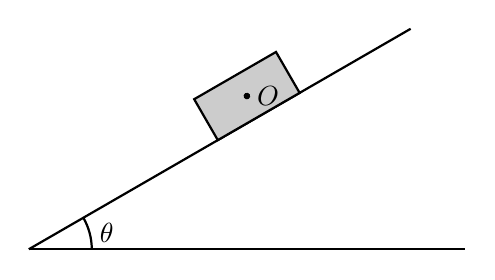
\begin{tikzpicture}[>=stealth, thick,scale=0.8]
  \draw (0,0) --(6.93,0) ;
  \draw (0,0)--(30:7);
  \draw [rotate=30, fill=black!20] (6.93/2,0) rectangle (6.93/2+1.5,0+.75);
  % \draw [rotate=30, ->, ultra thick] (6.93/2+.75,.75/2)-- (6.93/2+.75,.75/2-2.6) node [above]{$F_2$};
  % \draw [rotate=30, ->, ultra thick] (6.93/2+.75,.75/2)-- (6.93/2+.75,.75/2+2.6) node [above]{$N$};
  % \draw [rotate=30, ->, ultra thick] (6.93/2+.75,.75/2)-- (6.93/2+.75-1.5,.75/2)node [left]{$F_1$};
  % \draw [rotate=30, ->, ultra thick] (6.93/2+.75,.75/2)--node [right]{$G$} (6.93/2+.75-1.5,.75/2-2.6)node [below]{$G$};
  % \draw [rotate=30, dashed] (6.93/2+.75-1.5,.75/2)--(6.93/2+.75-1.5,.75/2-2.6)-- (6.93/2+.75,.75/2-2.6);
  \fill [rotate=30] (6.93/2+.75,.75/2) circle[radius=1.5pt] node [right]{$O$};
  % \draw [rotate=30](6.93/2+.75-1.5,.75/2-2.6+.75) arc(90:60:.75)node [midway,above]{$\theta$};
  \draw (0+1, 0) arc(0:30:1)node [midway,right]{$\theta$};
\end{tikzpicture}
\end{document}